\subsection{Sistemas de enclavamiento}

A modo de ejemplo, se ilustra en la Figura \ref{fig:enclavamiento_1} un sistema de cambios en una vía simple con bypass. Esto permite que dos formaciones puedan cruzarse en sentidos opuestos sin colisionar.

    \begin{figure}[h]
        \centering
        \includegraphics[width=0.5\textwidth]{example-image}
        \centering\caption{XXXXX.}
        \label{fig:enclavamiento_1}
    \end{figure}

Para evitar la colisión, se requiere un control seguro que evite que las formaciones avancen hacia secciones ya ocupadas por otras. También debe evitar que las formaciones avancen sobre los cambios cuando estos aún no han terminado de posicionarse en su lugar, lo que provocaría descarrilamientos. A este control se lo denomina sistema de enclavamiento y, en definitiva, impide que se produzcan configuraciones no seguras y controla los semáforos que habilitan o no los itinerarios de las formaciones. Una falla en un enclavamiento puede poner en peligro cientos de vidas humanas y generar gastos considerables. Por lo tanto, en el diseño del sistema de enclavamiento se deben cumplir estrictos parámetros de fiabilidad, disponibilidad, mantenibilidad y seguridad (RAMS).
    
\subsubsection{Bloqueo de máquina de cambios por ocupación}

\lipsum[1]
\includegraphics{example-image}
\lipsum[1]
\subsubsection{Requerimiento de rutas y bloqueo de cambios en ruta}

\lipsum[1]
\includegraphics{example-image}
\lipsum[1]
\subsubsection{Proteccion por aproximacion}

\lipsum[1]
\includegraphics{example-image}
\lipsum[1]
\subsubsection{Proteccion por solape}

\lipsum[1]
\includegraphics{example-image}
\lipsum[1]
\subsubsection{Doble recubrimiento}

\lipsum[1]
\includegraphics{example-image}
\lipsum[1]
\subsubsection{Liberación secuencial}

\lipsum[1]

    \begin{figure}[!h]
        \centering
        
\includegraphics[width=1\textwidth]{Figuras/secuencial_1}
        \centering\caption{Liberación secuencial.}
        \label{fig:secuencial_1}
    \end{figure}
    
\lipsum[1]

    \begin{figure}[!h]
        \centering
        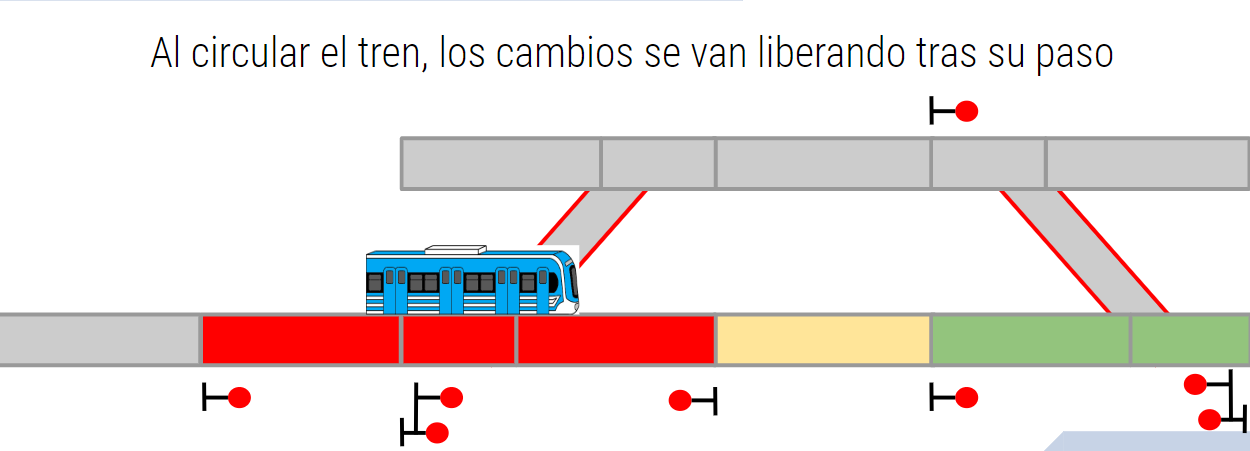
\includegraphics[width=1\textwidth]{Figuras/secuencial_2}
        \centering\caption{Liberación secuencial.}
        \label{fig:secuencial_2}
    \end{figure}
    
\lipsum[1]

    \begin{figure}[!h]
        \centering
        
\includegraphics[width=1\textwidth]{Figuras/secuencial_3}
        \centering\caption{Liberación secuencial.}
        \label{fig:secuencial_3}
    \end{figure}
    
\lipsum[1]

    \begin{figure}[!h]
        \centering
        
\includegraphics[width=1\textwidth]{Figuras/secuencial_4}
        \centering\caption{Liberación secuencial.}
        \label{fig:secuencial_4}
    \end{figure}
    
\lipsum[1]